\documentclass{article}
    \author{曹檑
    \ 2017310773}
    \title{快速聚类算法的性能分析}
\usepackage{xeCJK}
\usepackage{subfigure}
\usepackage{subfig}
\usepackage{indentfirst}
\setlength{\parindent}{2em}
\usepackage{graphicx}
    \setCJKmainfont{宋体}
\begin{document}
  \maketitle
    
    \section{对于论文的中的测试结果进行复现} 论文中给出了相当多的实验结果,我们选择了有代表性的Flame和Pathbased数据集进行测试
    \begin{figure}[!ht]
    \centering

    \begin{minipage}[c]{0.5\textwidth}
        \centering
      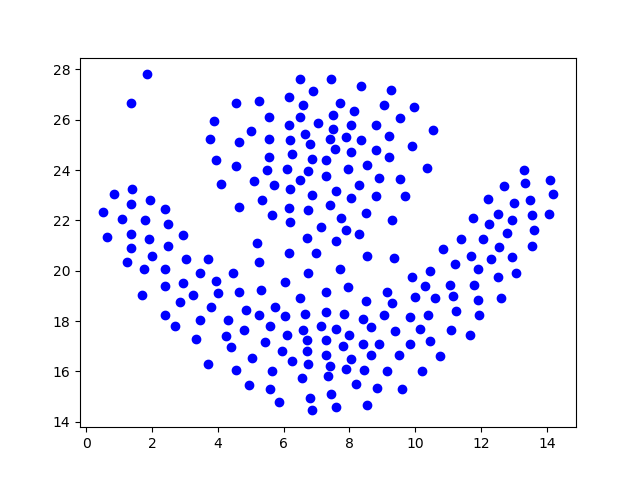
\includegraphics[height=1.5in,width=1.5in]{Flame}
      \caption{Flame数据集}\label{aa}
    \end{minipage}%
    \begin{minipage}[c]{0.5\textwidth}
        \centering
      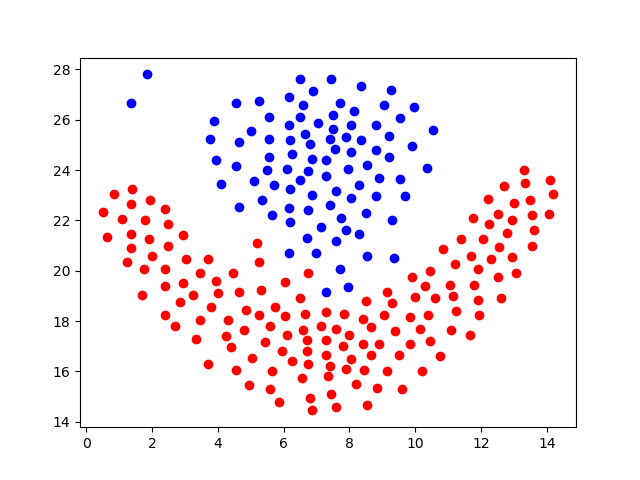
\includegraphics[height=1.5in,width=1.5in]{Flame2}
      \caption{Flame数据集实验结果}\label{aa}
    \end{minipage}
    \end{figure}
\begin{figure}[!htp]
\centering
    \begin{minipage}[c]{0.5\textwidth}
        \centering
      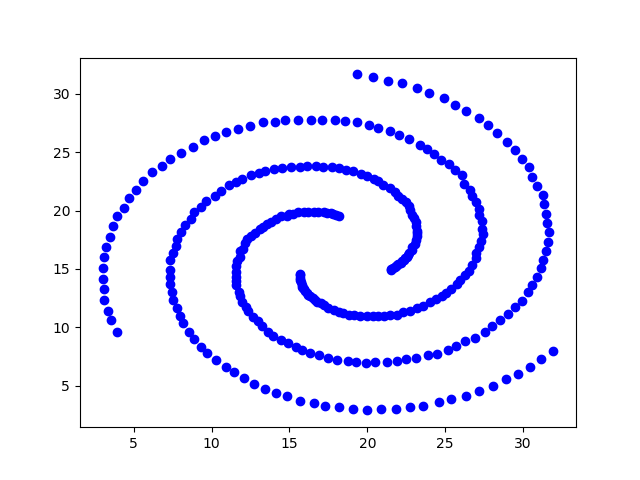
\includegraphics[height=1.5in,width=1.5in]{pathbased}
      \caption{Pathbased数据集}\label{aa}
    \end{minipage}%
    \begin{minipage}[c]{0.5\textwidth}
        \centering
      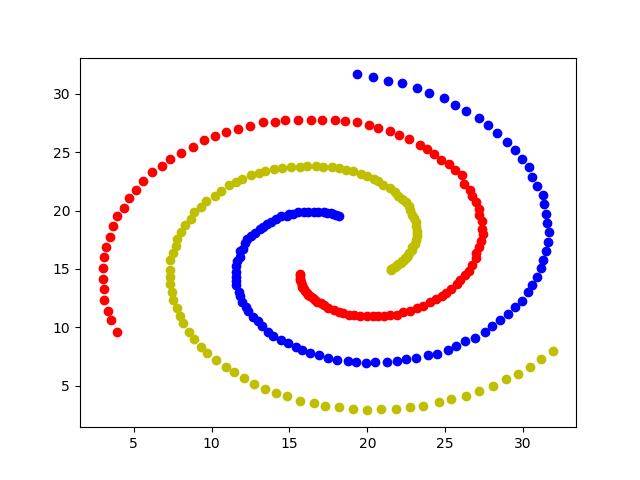
\includegraphics[height=1.5in,width=1.5in]{pathbased2}
      \caption{Pathbased数据集实验结果}\label{aa}
    \end{minipage}
\end{figure}
    Flame数据集由240个二维点组成,共有两类,实验结果中,240个点正确分对了237个,正确率98.8$\%$。
    
    实验结果表明,快速聚类算法对Flame算法十分有效。




    Pathbased由300个二维点构成,共有三类,实验结果中,所有分类都是正确的,正确率100\%。
    \section{与主流算法进行对比}
    共在六个数据集进行比较,每个数据集有1500个二维点。对比算法有MiniBath KMeans、Affinity Propagation、Mean Shift、Spectral Clustering、Ward、Agglomerative Clustering、DBSCAN、Birch、Gaussian Mixture。
    
    从测试集1和测试集2中我们可以看到,快速聚类算法依然不能很好的捕捉特殊几何图形的结构,比如圆形、弧线形,
   \begin{figure}[!ht]
\centering
    \begin{minipage}[c]{0.5\textwidth}
        \centering
      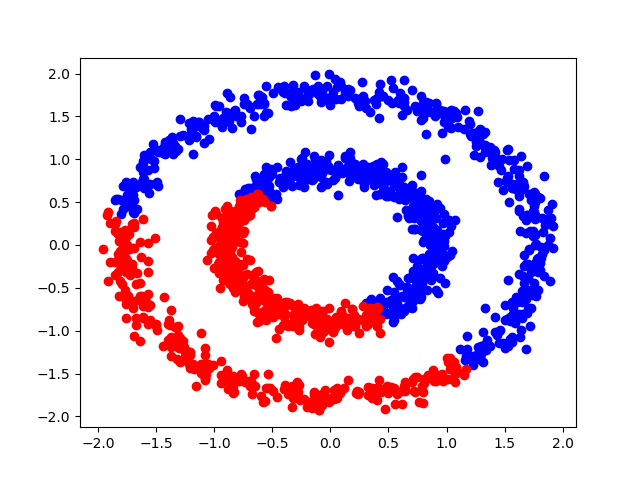
\includegraphics[width=2.5in]{ds1}
      \caption{测试集1数据集}\label{aa}
    \end{minipage}%
    \begin{minipage}[c]{0.5\textwidth}
        \centering
      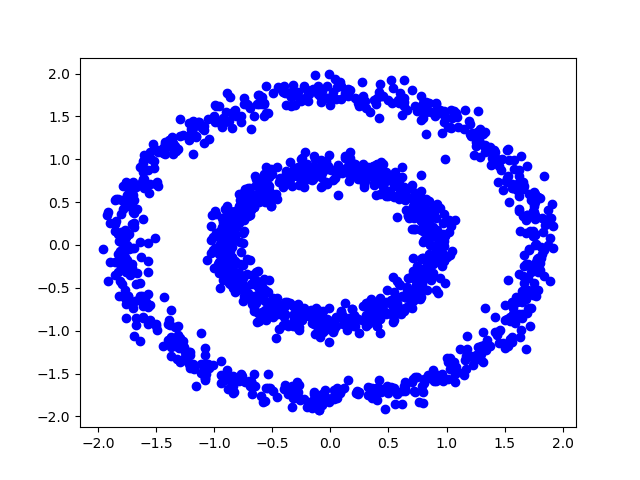
\includegraphics[width=2.5in]{ds12}
      \caption{测试集1数据集实验结果}\label{aa}
    \end{minipage}
\end{figure}


   \begin{figure}[!ht]
\centering
    \begin{minipage}[c]{0.5\textwidth}
        \centering
      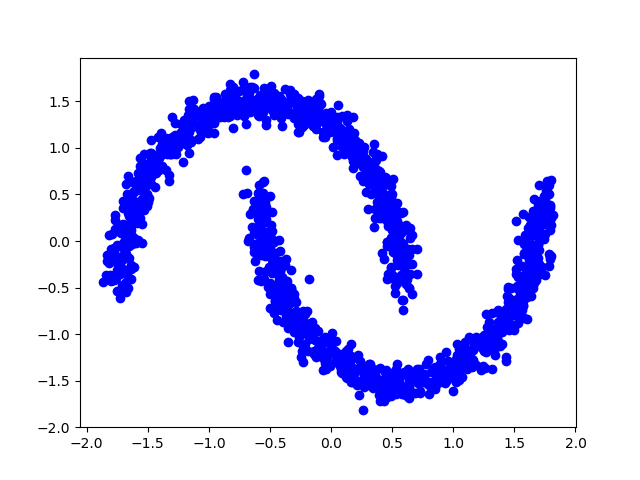
\includegraphics[width=2.5in]{ds2}
      \caption{测试集2数据集}\label{aa}
    \end{minipage}%
    \begin{minipage}[c]{0.5\textwidth}
        \centering
      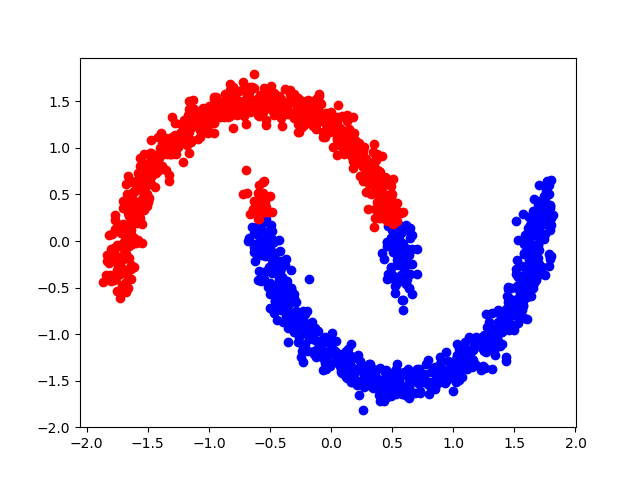
\includegraphics[width=2.5in]{ds22}
      \caption{测试集2数据集实验结果}\label{aa}
    \end{minipage}
\end{figure}


   \begin{figure}[!ht]
\centering
    \begin{minipage}[c]{0.5\textwidth}
        \centering
      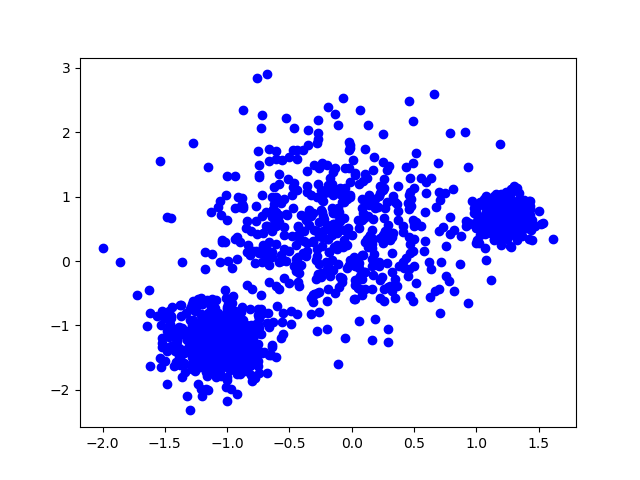
\includegraphics[width=2.5in]{ds3}
      \caption{测试集3数据集}\label{aa}
    \end{minipage}%
    \begin{minipage}[c]{0.5\textwidth}
        \centering
      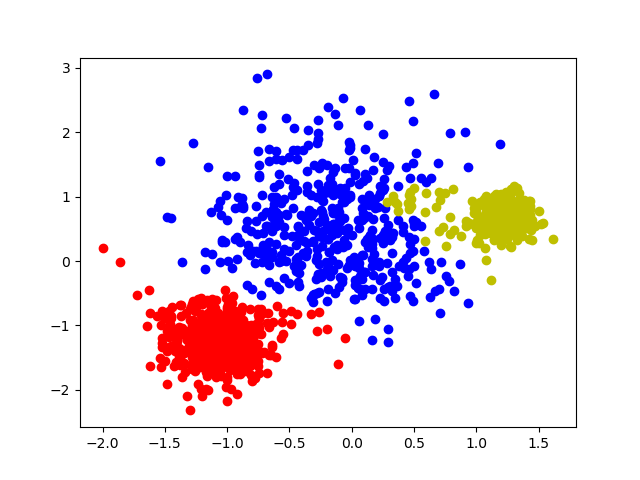
\includegraphics[width=2.5in]{ds32}
      \caption{测试集3数据集实验结果}\label{aa}
    \end{minipage}
\end{figure}



   \begin{figure}[!ht]
\centering
    \begin{minipage}[c]{0.5\textwidth}
        \centering
      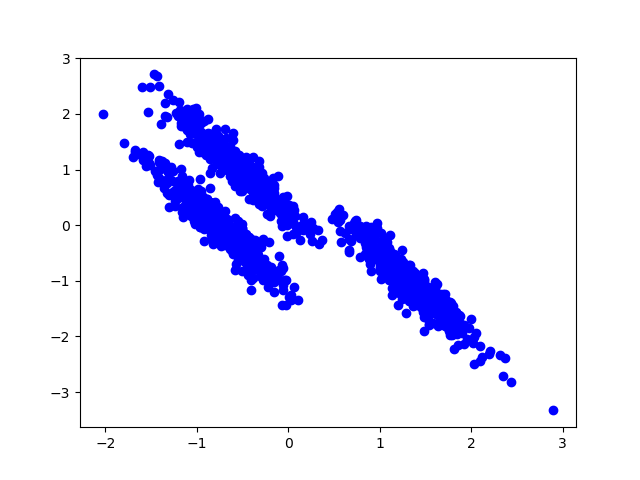
\includegraphics[width=2.5in]{ds4}
      \caption{测试集4数据集}\label{aa}
    \end{minipage}%
    \begin{minipage}[c]{0.5\textwidth}
        \centering
      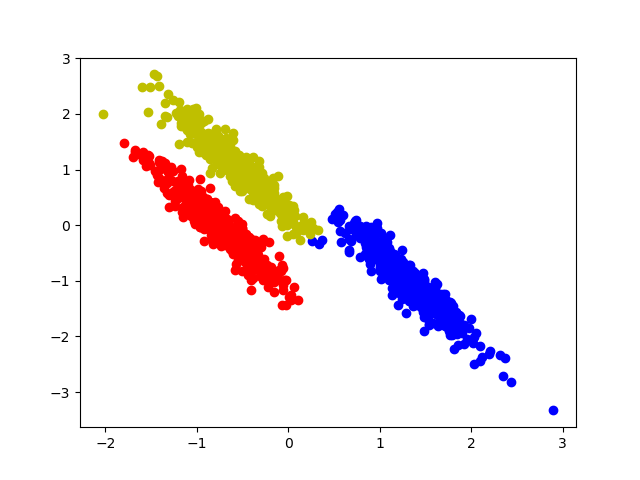
\includegraphics[width=2.5in]{ds42}
      \caption{测试集4数据集实验结果}\label{aa}
    \end{minipage}
\end{figure}

   \begin{figure}[!ht]
\centering
    \begin{minipage}[c]{0.5\textwidth}
        \centering
      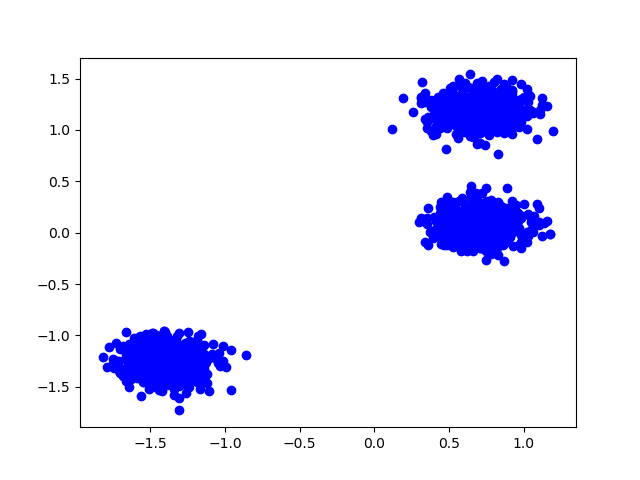
\includegraphics[width=2.5in]{ds5}
      \caption{测试集5数据集}\label{aa}
    \end{minipage}%
    \begin{minipage}[c]{0.5\textwidth}
        \centering
      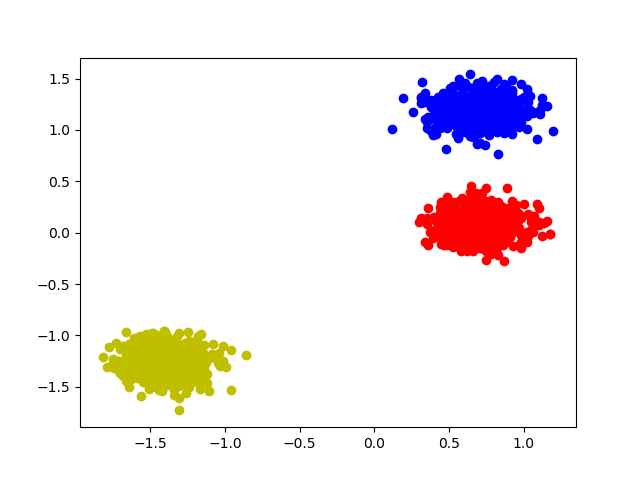
\includegraphics[width=2.5in]{ds52}
      \caption{测试集5数据集实验结果}\label{aa}
    \end{minipage}
\end{figure}

   \begin{figure}[!ht]
\centering
    \begin{minipage}[c]{0.5\textwidth}
        \centering
      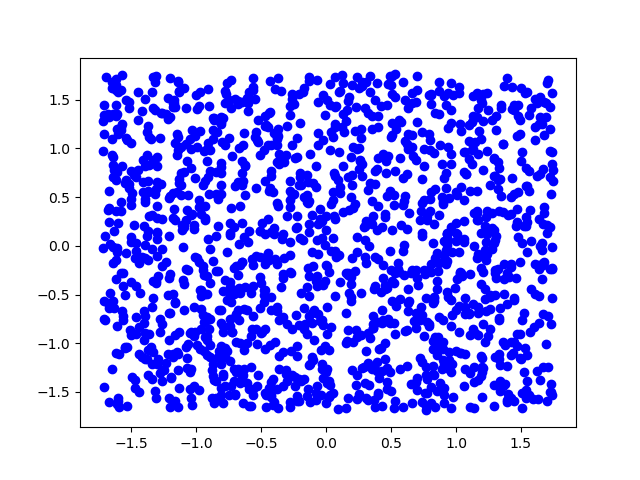
\includegraphics[width=2.5in]{ds6}
      \caption{测试集6数据集}\label{aa}
    \end{minipage}%
    \begin{minipage}[c]{0.5\textwidth}
        \centering
      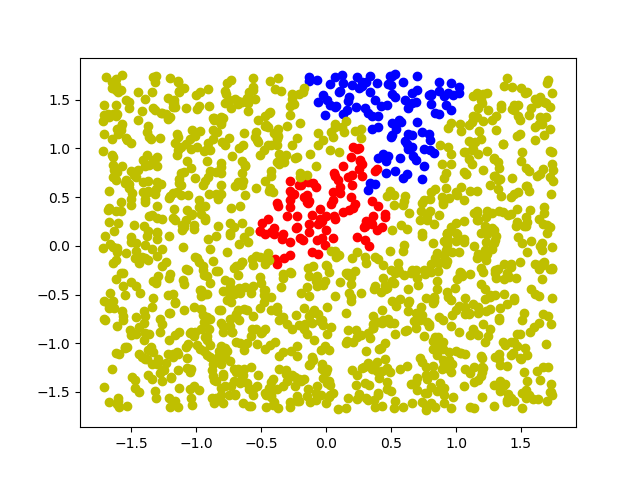
\includegraphics[width=2.5in]{ds62}
      \caption{测试集6数据集实验结果}\label{aa}
    \end{minipage}
\end{figure}

\begin{figure}[ht]

  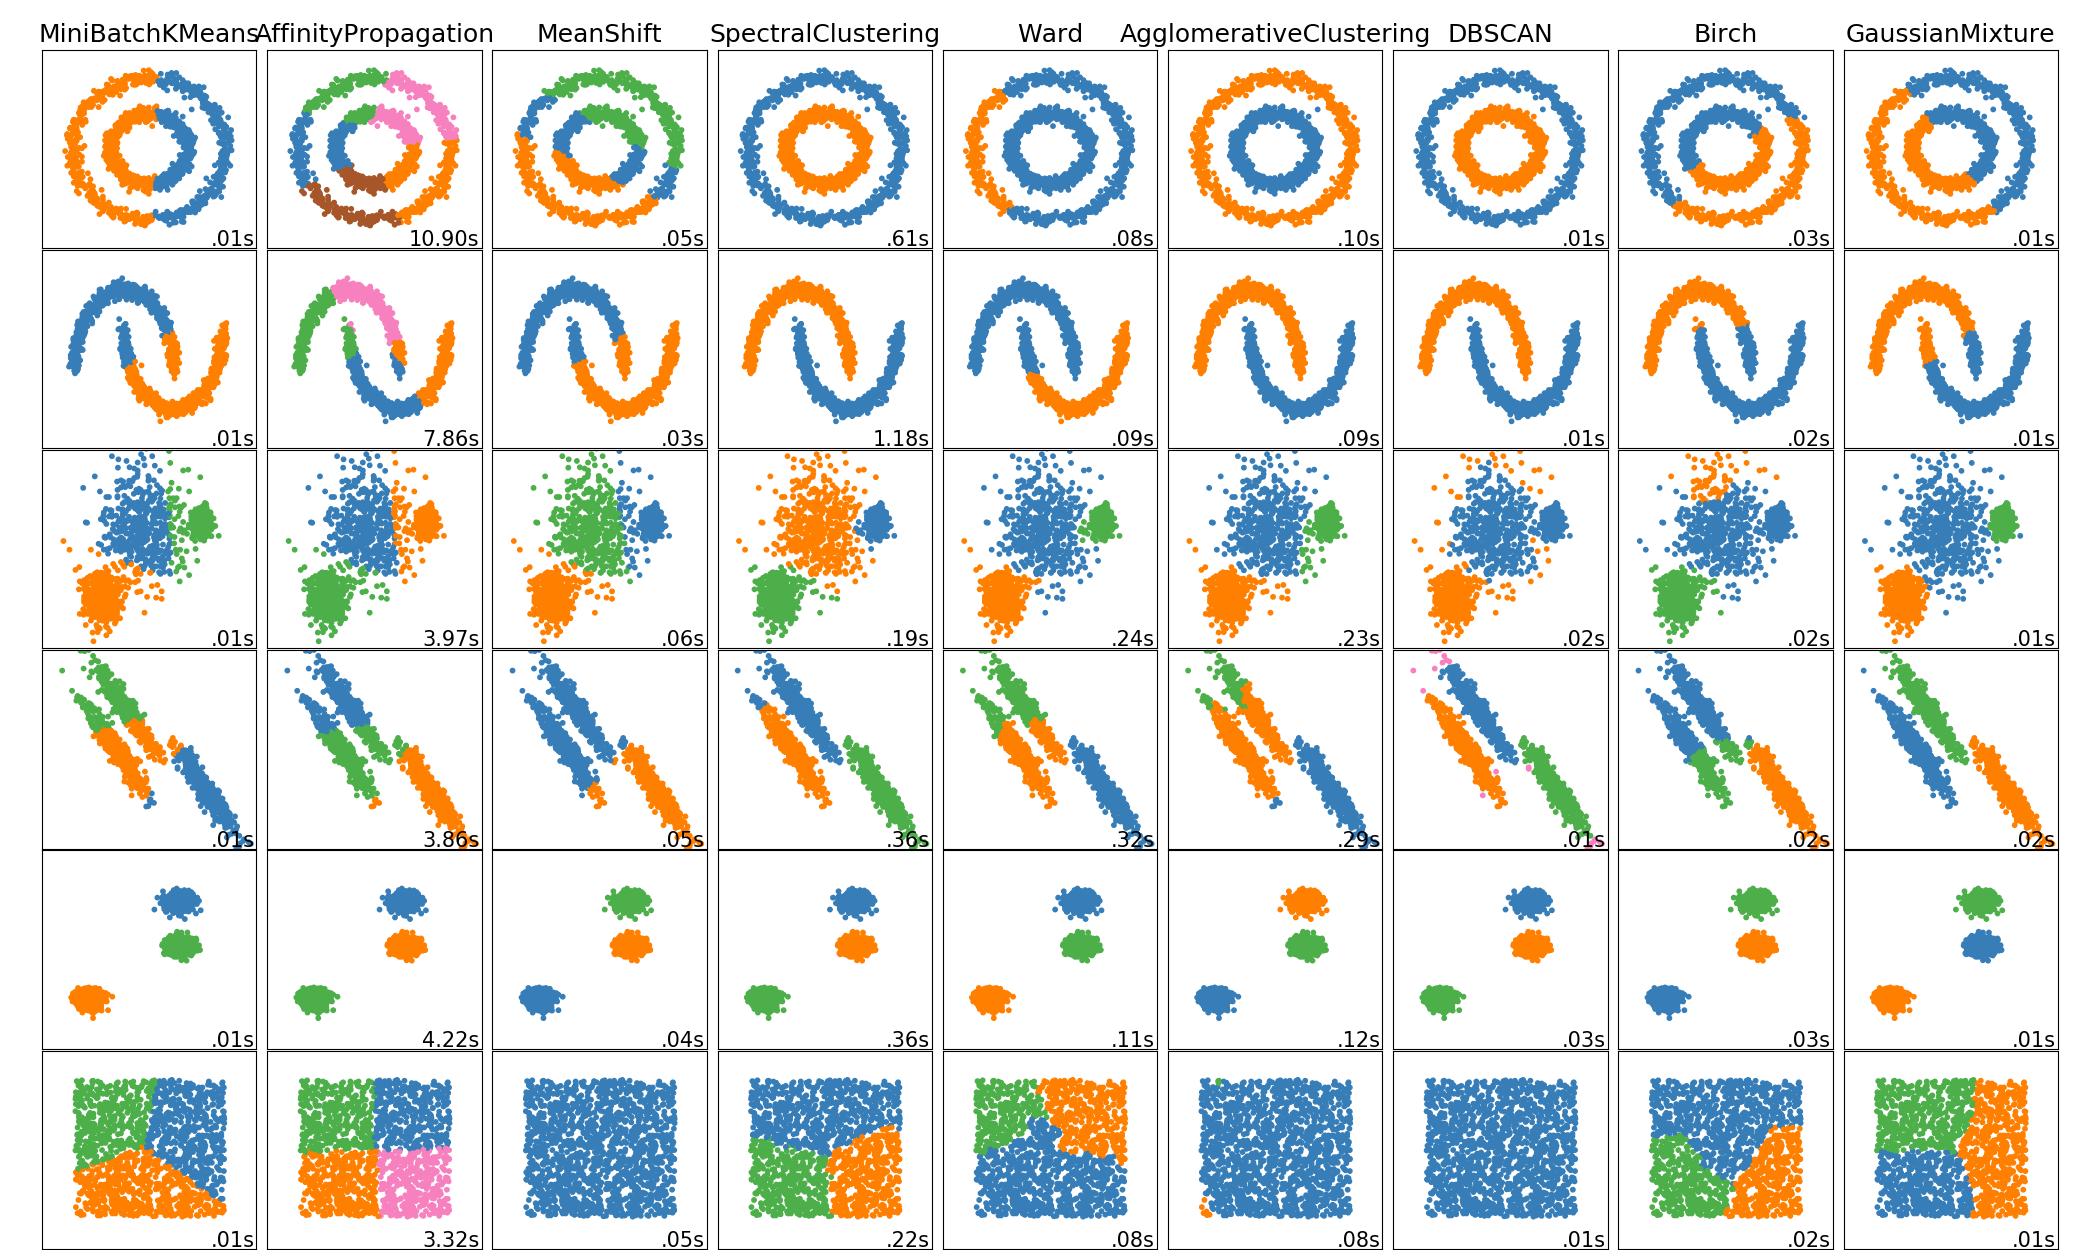
\includegraphics[width=5in]{test}
  \caption{其他算法对比实验结果}\label{aa}
\end{figure}



\end{document} 